\documentclass[a4paper]{article}

\usepackage[utf8]{inputenc}
\usepackage[T1]{fontenc}
\usepackage{textcomp}
\usepackage[italian]{babel}
\usepackage{graphicx}
\usepackage{siunitx}
\usepackage{float}
\usepackage{amsmath, amssymb}

\title{Relazione di Laboratorio 3 - Rimbalzi}
\author{Walhout Francesco - Iallorenzi Michele}

\begin{document}
    \maketitle

    \section{Introduzione}
    Una pallina elastica lasciata cadere da un altezza $h_0$ completa un certo numero di 
    rimbalzi, ad intervalli di tempo non costanti, prima di fermarsi.
    La sua energia meccanica varia di un fattore $ \gamma<0$ per ogni rimbalzo,
    per questo possiamo dire che l'altezza massima  $h_n$ raggiunta tra il rimbalzo
    $n$ e il rimbalzo $n+1$ è  data dalla formula:
    \begin{equation}
        \label{eq:altezza 1}
        h_n=h_0 \gamma^{n}
    \end{equation}
    Lo scopo dell'esperienza è quello di studiare il comportamento della pallina a partire
    dalle misure degli istanti di tempo dei rimbalzi, e confrontare le misure con i modelli
    matematici che predicono l'andamento delle altezze e la frequenza dei rimbalzi.

    \subsection{Strumenti utilizzati}
    \begin{itemize}
        \item Una pallina elastica
        \item Uno smartphone o dispostivo di registrazione audio
        \item Un metro a nastro
    \end{itemize}

    \section{Misure ed Analisi}
    \subsection{Misurazione}
    Vogliamo misurare i tempi analizzando una registrazione audio dei rimbalzi della pallina
    (nel nostro caso una pallina da ping pong),
    quindi è necessario posizionare lo strumento di registrazione per terra vicino
    a dove faremo cadere la pallina e assicurarsi che l'ambiente sia sufficientemente silenzioso.
    Per poter conoscere il valore di $h_0$, abbiamo utilizzato un metro a nastro per
    fare un segno su un muro ad $\SI{1}{\meter}$ dal suolo, e abbiamo poi lasciato cadere
    la pallina dall'altezza del segno, assicurandoci di lasciare spazio a sufficienza per evitare
    che la palla si scontri con il muro o con lo strumento di misurazione.
    Abbiamo registrato il rumore dei rimbalzi della pallina avviando
    la registrazione poco prima di lasciar cadere la pallina e arrestandola subito dopo l'ultimo rimbalzo.
    \begin{figure}[ht!]
        \centering
        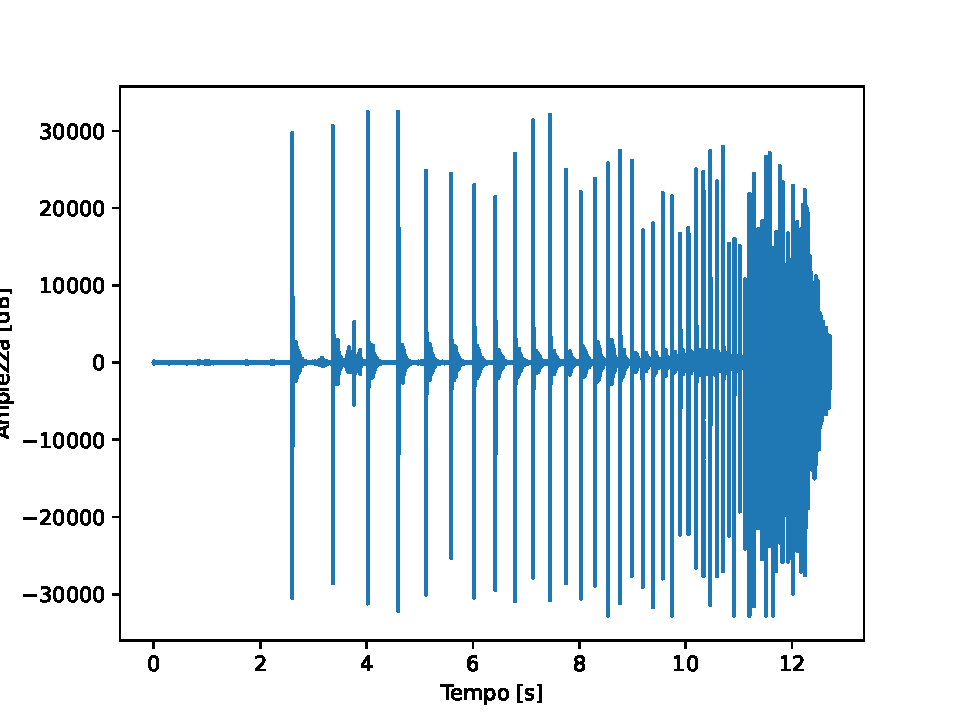
\includegraphics[width=0.8\textwidth]{extra/audio_rimbalzi.pdf}
        \caption{Grafico delle ampiezze della registrazione}
        \label{fig:ampiezze}
    \end{figure}

    \subsection{Campionamento}
    Osservando il grafico delle ampiezze delle registrazioni fatte, si nota che ciascun rimbalzo
    ha un picco iniziale ben definito e una coda più lunga. 
    Abbiamo scelto di campionare come istante di impatto il picco maggiore all'inizio di ciascun rimbalzo,
    ignorando la coda.\\
    Per effettuare il campionamento abbiamo scritto un programma in python che individua
    gli intervalli di tempo in cui l'ampiezza della traccia audio sale sopra ad un threshold
    arbitrario e per ciascun intervallo restituisce il punto centrale come istante d'impatto.
    Come incertezza abbiamo utilizzato metà della durata del picco audio più lungo,
    che risulta essere $\SI{0.002}{\second}$.\\
    I dati così ottenuti sono riassunti nella tabella \ref{tab:rimbalzi}, oltre il
    cinquantesimo rimbalzo diventa difficile distinguere i picchi perciò
    non abbiamo campionato ulteriori impatti.
    \begin{table}[ht!]
        \centering
        \begin{tabular}{ll|ll|ll}
            Rimbalzo & Istante [\si{s}] & Rimbalzo & Istante [\si{s}] & Rimbalzo & Istante [\si{s}]\\
            \hline
            \hline
            1&2.604&18&9.191&35&11.365\\
            2&3.366&19&9.385&36&11.441\\
            3&4.022&20&9.568&37&11.523\\
            4&4.600&21&9.738&38&11.581\\
            5&5.119&22&9.900&39&11.647\\
            6&5.591&23&10.054&40&11.708\\
            7&6.025&24&10.198&41&11.767\\
            8&6.423&25&10.336&42&11.822\\
            9&6.791&26&10.465&43&11.875\\
            10&7.133&27&10.588&44&11.925\\
            11&7.452&28&10.703&45&11.972\\
            12&7.750&29&10.813&46&12.018\\
            13&8.030&30&10.918&47&12.060\\
            14&8.292&31&11.017&48&12.100\\
            15&8.538&32&11.111&49&12.138\\
            16&8.769&33&11.201&50&12.175\\
            17&8.986&34&11.285&
        \end{tabular}
        \caption{Istanti di ciascun rimbalzo della pallina. L'incertezza è di $\SI{0.002}{\second}$.}
        \label{tab:rimbalzi}
    \end{table}
    \subsection{Elaborazione dei dati}
    Utilizzando le leggi della cinematica per corpi in moto uniformemente accelerato,
    e ignorando quindi l'attrito dell'aria ed altre perturbazioni, si può dimostrare la
    seguente formula:
    \begin{equation}
        \label{eq:altezza 2}
        h_n=-\frac{1}{8}g\left( t_{n+1}-t_{n} \right) ^2
    \end{equation}
    che ci permette di calcolare le altezze a partire dai dati di cui disponiamo.\\
    Abbiamo quindi fatto un grafico di disperzione ed un fit di questi dati utilizzando
    la funzione curve\_fit della libreria scipy, il risultato è mostrato in figura \ref{fig:altezze}.
    \begin{figure}[ht!]
        \centering
        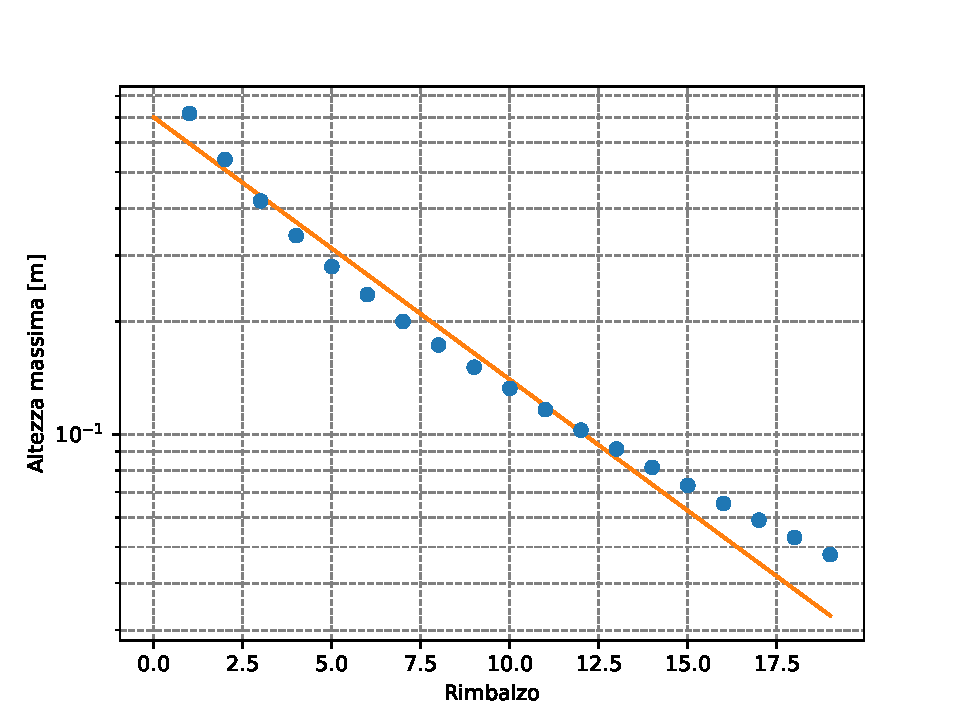
\includegraphics[width=0.8\textwidth]{extra/altezza_rimbalzi.pdf}
        \caption{Grafico di disperzione delle altezze massime di ciascun rimbalzo,
        con best fit e grafico dei residui.}
        \label{fig:altezze}
    \end{figure}
    Osservando il grafico dei residui ottenuto si nota che i punti che più si discostano
    dal modello utilizzato sono i primi, ovvero i rimbalzi effettuati da un altezza 
    notevolmente maggiore rispetto ai successivi.\\
    Abbiamo quindi rietenuto opportuno eseguire un ulteriore fit ignorando i primi $10$ rimbalzi
    per verificare se gli urti a velocità più moderate si adattassero meglio al modello
    in considerazione, il risultato è mostrato in figura \ref{fig:altezze_2}.\\
    Per entrambi i fit, i valori ottenuti per le altezze iniziali $h_0$,
    il fattore $\gamma$ e le relative incertezze sono mostrati in tabella \ref{tab:fit}
    \begin{figure}[ht!]
        \centering
        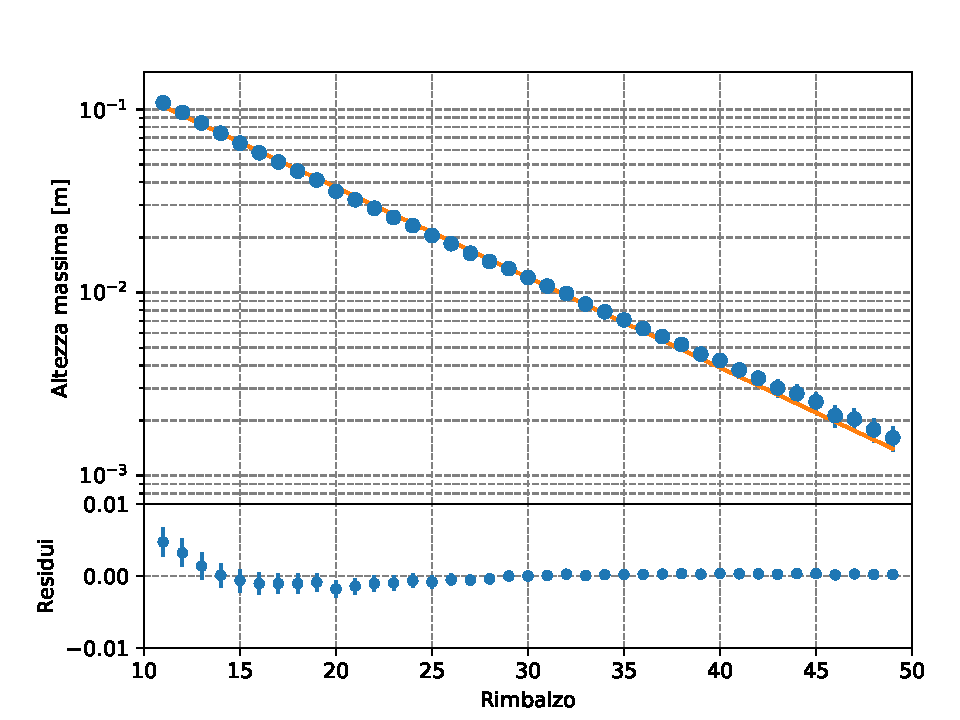
\includegraphics[width=0.8\textwidth]{extra/altezza_rimbalzi[10:].pdf}
        \caption{Grafico di disperzione con fit degli ultimi 40 rimbalzi della pallina.}
        \label{fig:altezze_2}
    \end{figure}
    \begin{table}[ht!]
        \centering
        \begin{tabular}{ll|ll}
            \multicolumn{2}{c|}{Fit su 50 rimbalzi} & \multicolumn{2}{c}{Fit su 40 rimbalzi} \\
            \hline
            \hline
            $h_0$ [\si{\m}] & 0.627 & $h_0$ [\si{\m}] & 0.116\\
            $\sigma_{h_0} [\si{\m}]$ & 0.024 & $\sigma_{h_0} [\si{\m}]$ & 0.001\\
            $\gamma$ & 0.8634 & $\gamma$ & 0.8929\\
            $\sigma_{\gamma}$ & 0.0036 & $\sigma_{\gamma}$ & 0.0007
        \end{tabular}
        \caption{Parametri ottenuti dai fit.}
        \label{tab:fit}
    \end{table}
    \section{Conclusioni}
    Osservando i due diversi fit eseguiti, si può subito notare che in generale il
    modello esponenzionale non descrive adeguatamente il comportamento della pallina,
    tuttavia considerando solo urti ad altezze e quindi velocità sufficientemente basse,
    i dati si adattano molto bene al modello scelto. Per determinare, nel caso generale,
    quale sia un altezza iniziale sufficientemente bassa da rendere trascurabile l'errore
    commesso dal modello esponenziale sarebbe necessario studiare un modello più generale
    che descriva più precisamente la perdita di energia della pallina e permetta quindi
    di determinare l'errore commesso dal modello esponenziale.\\
    Possiamo ipotizzare che le cause di questo errore siano la maggiore deformazione della
    pallina causata dalla velocità degli urti e il maggiore attrito con l'aria a cui la 
    pallina va incontro muovendosi a velocità maggiori lungo traiettorie più lunghe.\\
    Per quanto riguarda i valori ottenuti per le altezze iniziali $h_0$ per il primo fit
    si è ottenuto un valore inferiore di quello misurato, anche se considerassimo
    qualche centimetro di incertezza sulla nostra misura.
\end{document}
